\chapter{Implementation of the mem-HNN}

\section{Objectives and research methodology}
Upon establishing the precise research methodology, this chapter delves into the implementation of the Simulator Pipeline.
First, the analysis phase of the \ac{DSR} process is executed to establish a model of the Simulator Pipeline,
which the requirements and conditions can be derived from. 
Next, a practical prototype is developed in iterative design cycles to fulfill the target requirements.
In the evaluation phase, the simulator pipeline is used to assess the performance of the \ac{mem-HNN} 
in the training of an exemplary machine learning workload. 
This thesis utilizes performance metrics collected from the simulation to address the central research question, which explores potential speed and efficiency enhancements of the \ac{mem-HNN} compared to digital computers.


\section{Analysis phase}
\subsection{General conditions}

Following the first phase of the \ac{DSR}-cycle described in Chapter 3, the research outline is initially established from which the requirements for the simulator pipeline are derived.\footcite[cf.][278-279]{oesterleKonsortialforschung2010}
This analysis begins by describing the general conditions specified in Section 3.1.
Hereby, general conditions are permanent design decisions that are used as the foundation for the implementation of the Simulator Pipleine.
The underlying motivation hereby is to research if the known proof of concepts is feasible on the complete \ac{mem-HNN}
and evaluate if that brings an actual acceleration, which is equivalent to answering the research question of this thesis. 

The implementation is executed in the programming language Python since it offers a variety of third-party libraries that are useful 
for machine learning that is state of the art, like PyTorch, Scikit learn etc..\footcite[cf.][306-307]{DiscreteContinuousModels}
Furthermore, Scikit Learn is chosen as a machine learning library since it is one of the industry standards for classical machine learning, has a broad variety of features in terms of \ac{BM}s
and has a lower learning curve compared with e.g. Tensorflow.\footcite[cf.][5-6]{raschkaMachineLearningPython2020}
For simplicity and to save time, a \ac{RBM} is used as a test case with handwritten digit classification as workload.

The complete \ac{mem-HNN} is being simulated based on a design that has been developed by the Forschungszentrum Jülich and HPE.\footcite[cf.][3-4]{hizzaniMemristorbasedHardwareAlgorithms2023}  
This design describes an \ac{ASIC} design that realizes the noisy Hopfield Network shown in figure\ref{ModellHMM}.
It includes an energy model based on low-level circuit simulations, which can derive the average energy consumption per clock cycle of the \ac{mem-HNN}.
In addition to that, the model includes latency estimations of the \ac{mem-HNN} to perform a full iteration. 
This simulation approach is chosen as the device is still under development and hardware devices are not available yet.
Nonetheless, the complete hardware can be realized in software without compromising its functionality.
Such a simulation-based performance evaluation is quite common in the \ac{ASIC} design flow.\footnote{cf.\cite{raoUltimateGuideASIC}, p. 1; cf.\cite{ASICDesignFlow}, p. 1}
An in-depth explanation of this model is out of scope for this thesis but core parameters are explained to understand the gathered energy values.
Lastly, the simulation is performed on a notebook.
Due to the limitations of the built-in \ac{CPU}\footnote{\texttt{Intel i7-10610U, 1.80GHz, 2304 MHz, 4 Cores, 8 Logical Processors}}, efficient coding is required to ensure simulations are performed within an acceptable timeframe.

\subsection{Requirements}

To evaluate the performance of \ac{mem-HNN}s in training and inference of \ac{BM}s, a full simulator pipeline has to be modeled.
In Fig.\ref{Overall architecture} the envisioned model is shown, in which an \ac{mem-HNN} chip can be used to implement \ac{BM}s.
Here, a digital computer is used to implement and train machine learning models on various datasets.
The \ac{mem-HNN} chip is then used to perform the sampling during the \ac{BM} inference or training.
Training and inference on this system then involves the following five steps, which are handled by different components and describe the interaction between the digital computer and the analog \ac{mem-HNN} chip:
\begin{figure}[H]
    \centering
    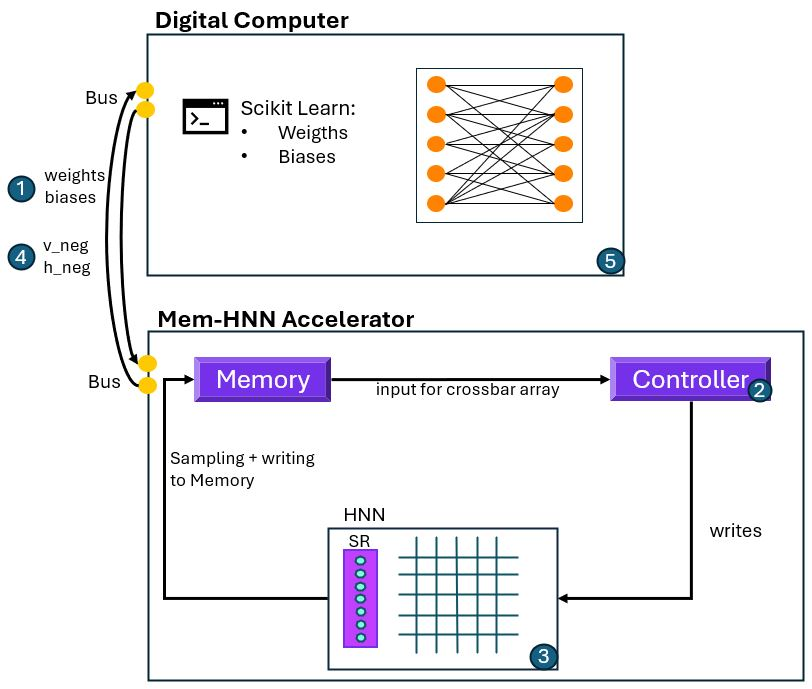
\includegraphics[width=0.80\linewidth]{graphics/Analysemodell.JPG}
    \caption{proposed solution architecture}
    \label{Overall architecture}
\end{figure}
\textbf{1.} initializes the machine learning model (neural network) including setting the weights and biases of the \ac{BM}. 

\textbf{2.} starts with the transfer of the weights and biases to the \ac{mem-HNN} accelerator via a bus system. 
The local memory saves the data and forwards them to the controller. 
The controller is able to program the memristors in the crossbar array. 

\textbf{3.} is the Hopfield Neural Network (HNN), which contains the memristor crossbar array and the state register (SR).
Here, \ac{mem-HNN} performs a pre-defined amount of iterations, where a sample configuration is stored in the on-chip memory after each iteration.\footcite[cf.][18]{caiHarnessingIntrinsicNoise2019}
The state register includes the current neuron configuration and can lock and unlock specific neurons so that it is possible to update neurons synchronously.\footcite[cf.][18]{caiHarnessingIntrinsicNoise2019}
This enables the possibility of the promising N/2 update strategy.

\textbf{4.} After the \ac{mem-HNN} has performed all iterations, the stored sample configurations
of the visible \(v_{neg}\) and the hidden \(h_{neg}\) neurons are transferred back to the digital computer via the bus system.

\textbf{5.} With the sample configurations, the digital computer calcualtes the activation probabilities and performs
the updates to the weights and biases according to the training rule in equation\ref{Update_weights}.
These training updates are repeatedly performed starting again from step 2 until the model achieves sufficient performance.
Furthermore, the model can be evaluated in its performance in terms of chosen metrics like prediction accuracy or negative likelihood etc..

In the Simulator Pipeline the behavior of the \ac{mem-HNN} in fig.\ref{Overall architecture} is mimicked, where the simulator acts as a drop-in replacement until hardware devices become available.
The simulator models the behavior of the chip so that performance predictions are possible long before a hardware device can eventually be used.
Here, it is important to stress that the current hardware model described in the previous section currently does not contain modeling results for the on-chip memory, the controller and the bus system.
The simulator is therefore solely focused on modeling the sampling step 3.
With more modeling results becoming available, accurate simulations of steps 2 and 4 can be added to the simulator.
The next step is to derive the requirements and establish the research outline.
The aim of generating requirements is to generate good quality, requirements that offer an acceptable level of risk to start the project.\footcite[cf.][11]{ebertSystematischesRequirementsEngineering2008}
These requirements need to cover the functions of the \ac{mem-HNN}, which then must be implemented by the respective software components.
Also, requirements may evolve over time and require adjustments when outcomes differ from initial expectations.
As a result, considering the research question and objectives, the following software requirements emerged:

\textbf{Digital Computer}
\begin{itemize}
    \item Initialize a \ac{BM}
    \item Utilization of any training data
    \item Initializing of other ML models that are used in conjucntion with the \ac{BM} for evaluation
    \item Training of the \ac{BM} with either Gibbs Sampling or Metropolis Hasting
    \item Setting individual parameters: sampling steps, training iterations, noise level, learning rate 
    \item Evaluation of the model's performance using prediction accuracy and negative likelihood
\end{itemize}
\textbf{Simulated Mem-HNN Accelerator}
\begin{itemize}
    \item Using any \ac{BM} as input
    \item Implementing the noisy Hopfield Neural Network update mechanism described in \ref{noisy_update_HNN_formula}
    \item Return sampled output of the neuron configurations 
    \item Selectively switching between the N/2 half updating method instead of single spin updates described in 2.4
    \item Simulation of computation speed (throughput) and energy consumption of the \ac{mem-HNN} chip
\end{itemize}
Furthermore, the Python program should be split logically into different modules and components to enable well-structured code. 
With set requirements, it is now possible to begin the iterative design and evaluation cycle by focusing on some requirements per iteration.

\section{First Design and Evaluation phase}

This \textbf{Design phase} has the goal of implementing the parts of the simulator pipeline that are executed 
on the digital compuer in fig.\ref{Overall architecture} requirements.
Accordingly, the resulting prototype of this iteration has to satisfy all requirements listed under digital computer in section 4.2.
The implementation is verified with a test case based on the classification of handwritten digits.
The first step in the described prototyping methodology within 3.3 is to perform the systemic analysis to categorize the prototype.
In the realm of prototyping, the following categorizations are made: the prototype type (1) is computational, and its fidelity level (2) is high, as it aims to model all functionalities closely to reality.
Furthermore, the complexity (3) is considered moderate because not all hardware components can be modeled in software.
Additionally, the scale (4) remains constant, and there are multiple iterations (5) executed sequentially to train and infer the \ac{RBM}.
This process of categorizing the prototype helps to make prototypes comparable as prototyping can be used very vaguely.
The second step is to set up the Scikit Learn machine learning library as explained in 4.2.
Scikit Learn includes built-in models for \ac{BM}s that enable rapid development also including popular datasets, delivering results that are comparable with those found in literature.
This is useful to answer the research question in a timely manner.
Especially, the test case used for the \ac{BM} is based on an example of the official scikit learn documentation.\footcite[cf.][1]{RestrictedBoltzmannMachine}

The following task is to set parameters like the learning rate, iterations, and size of the hidden layer. 
With having a look in the literature and through testing a learning rate of \(0.2\), 10 training epochs with 72 iterations in one epoch, and a hidden layer of 100 neurons is chosen.\footnote{cf.\cite{hintonPracticalGuideTraining2012}, p. 11-12; cf.\cite{bohmNoiseinjectedAnalogIsing2022}, p. 1}
The size of the visible layer is automatically recognized by Scikit Learn, so for example 64 corresponds with 8x8 images of a dataset.
Also, the dataset implementation can be customized as needed, such as for a breast cancer classification workload.

The training of the \ac{RBM} is performed in the \texttt{.fit} method and for the functionality to select the preferred sampling algorithm an additional sampling method needs to be added.
This process includes modifying the \texttt{\_rbm.py} file in the basic scikit learn library.
The predefined sampling method is Gibbs sampling and there is no option to access metropolis hasting within the basic library. 
Therefore, the metropolis hasting algorithm, explained in 2.2.3 needs to be manually implemented.
The according adjustments are included from the code availability of a paper.\footcite[cf.][11-12]{bohmNoiseinjectedAnalogIsing2022}
This decision is made because the algorithm used there is the original metropolis algorithm by Metropolis et.al..\footcite[cf.][1087-1092]{metropolisEquationStateCalculations1953}
Furthermore, the implementation is performant with many numpy functions. 
To utilize this sampling method, some minor adjustments are made for user-friendliness. 
First, one function is fixed that has a small error, which produces an erroneous empty configuration as the first sampling iteration. 
The user-friendliness is achieved by introducing a new parameter \texttt{sampling\_method} that dynamically allows for change of the sampling method. 
Another change is the approach of evaluating the performance of the neural network after an x amount of iterations to measure its performance on the test data while training.
A complete code overview of the metropolis hastings sampling algorithm can be found in the \texttt{mcmc2.py} file as part of the digital delivery with all
adjusted methods for the training of the \ac{RBM} in \texttt{\_rbm.py}, while the overall execution takes place in the \texttt{playground.py}.

To evaluate the results and functionalities the \textbf{Evaluation phase} in this iteration validates the functionalities through a training of the \ac{RBM}. with each sampling method and extract their prediction accuracy.
Scikit Learn offers a variety of datasets that are already in a polished format, and ready to use. 
The decision is to use a classification workload of handwritten digits as a test case for validating the implementation.
One reason for this is that the ``load digits dataset'' is similar to the well-known MNIST dataset representing an industry-standard problem, but has a smaller resolution of 8x8 pixels and features around 1800 samples that can be categorized into 10 classes (integers 0-9).\footcite[cf.][1]{SklearnDatasetsLoad_digits}
The second reason is that the workload is already optimized and therefore can deliver relevant data for the research question.
In this case, additionally, a nudging of the data is chosen to create more samples, by a factor of five, and to bring more complexity to the workload. 
The split in the dataset is selected to be divided into the conventional 80\% training data and 20\% test data.\footnote{cf.\cite{charithaTypeIIDiabetesPrediction2022a}, p. 1-2; cf.\cite{supriAsianStockIndex2023}, p. 1}
For training, an \ac{RBM} is selected as the feature extractor and paired with a logistic regression classifier for prediction, thereby establishing a cohesive pipeline.
The following figure\ref{CD_baselines} shows the training results using the Gibbs sampling approach. 

\begin{figure}[H]
    \centering
    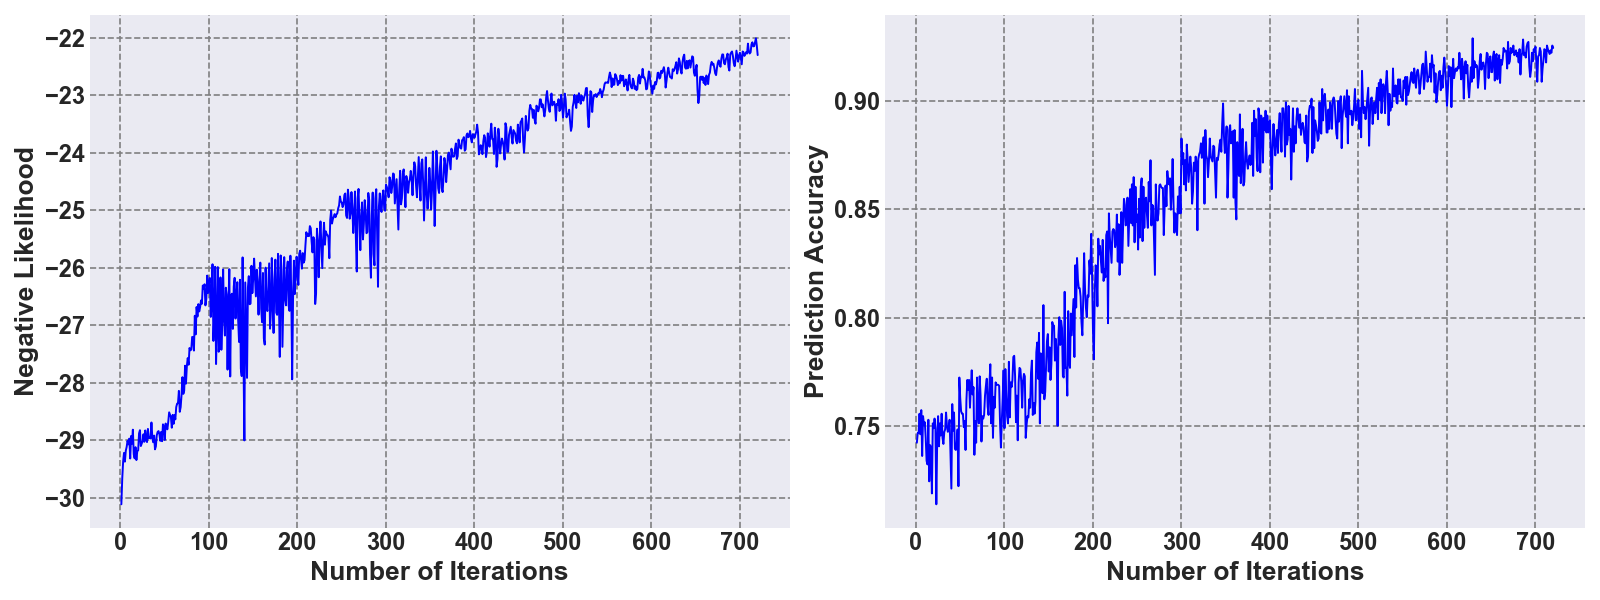
\includegraphics[width=0.9\linewidth]{graphics/CD_combined_plot.png}
    \caption{Gibbs sampling baselines}
    \label{CD_baselines}
\end{figure}
The right plot shows that the initial prediction accuracy starts at 75\%, akin to that of just a single linear regression model.
This suggests that the untrained \ac{RBM} at the input of the classifier initially does not affect the model's classification performance.
Data points are collected after every iteration across the span of 720 iterations. 
After 650 iterations the accuracy slowly stagnates and has a maximum prediction accuracy
of 92.29\%. 
In the left plot the negative likelihood, which is a measure of how well a statistical model represents the observed data.
When training a model the aim is to minimize the negative log-likelihood, which means that the model maximizes the probability of generating the observed data.
Hence, it is visible that in the beginning, the model learns more rapidly and steadily grows its knowledge with some smaller break-ins at the end.
The best value is a negative likelihood of -22.01.
\begin{figure}[H]
    \centering
    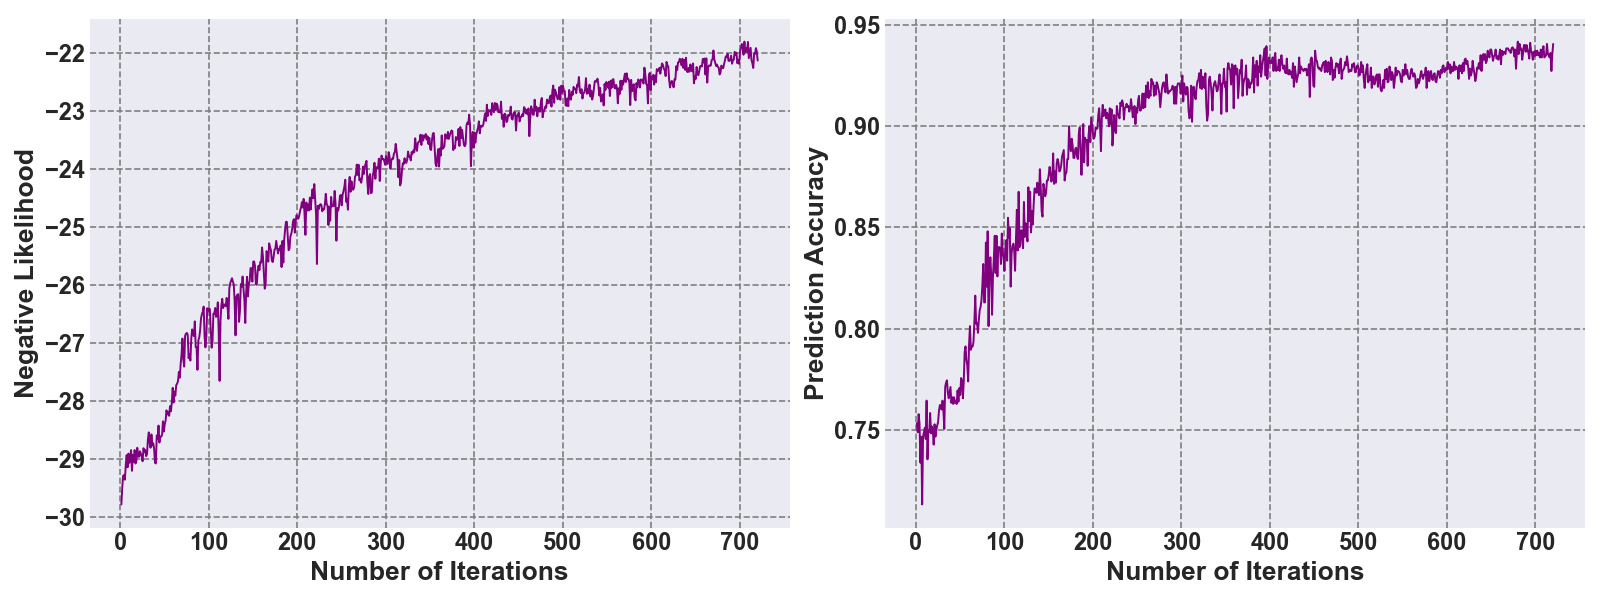
\includegraphics[width=0.9\linewidth]{graphics/metropolis_combined_plot.png}
    \caption{Metropolis sampling baselines}
    \label{metropolis_baselines}
\end{figure}
In contrast, the fig.\ref{metropolis_baselines} used the sampling algorithm of metropolis hasting to train the \ac{RBM}.
Noteworthy is that the prediction accuracy in the right plot has a faster increase in the beginning but already starts to stagnate at around 400 iterations. 
Here, the maximum prediction accuracy achieves 94.15\%. 
The negative likelihood is also growing faster than in Gibbs sampling and exhibits less variability showing a more continuous learning rate.
Here, the best negative likelihood value is -21.80.
Furthermore, to validate the accuracy of the results, they are compared against similar results to those from the literature.\footnote{cf.\cite{bohmNoiseinjectedAnalogIsing2022a}, p. 5; cf.\cite{RestrictedBoltzmannMachine}, p. 1}
Therefore, a good agreement is visible, suggesting that the implementation produces valid results and can thus be considered correct.
As a result, with each sampling method successfully undergoing training, all the functionalities can be proven right and the prototype can be passed 
into the next design iteration.
The gathered data can later on be used as a baseline against the desired new updating method of sampling with a Hopfield Network.


\section{Second Design and Evaluation phase}

This \textbf{design phase} iteration has the goal of implementing the simulator for \ac{mem-HNN} chip shown in fig.\ref{Overall architecture}.
The functionality of this chip is that of a noisy Hopfield Neural Network, which has previously been described in 2.4.4.
The update mechanism is based on the update formula in eq.\ref{noisy_update_HNN_formula}, where noise is injected to imitate the stochastic behavior of the neurons.
Hence, a \ac{BM} can be modeled by correctly tuning the noise of the Hopfield Neural Network.
The following subfunctionalities need to be established: drawing random neurons to update,
correct injection of the Gaussian noise scale, calculating the weighted sum,
comparing the weighted sum + bias + noise against the threshold and saving the new neuron configuration.
Furthermore, the possibility of selectively switching between the N/2 half-updating method instead of single spin updates
is to be included in this design phase. 
Hence, this iteration aims to break new ground as it involves implementing the Simulator Pipeline, which has not yet been validated and integrates the noisy Hopfield Network with the capability for N/2 half updating.

The Hopfield Network is initialized with a size of just one neuron and a sampling iteration counter of \(1500\) iterations with a thermalization of \(100\) sampling steps before 
the neuron is updated.
Thermalization is included to allow the network to perform independent sampling steps and get into a flow to ensure unbiased sampling steps.
The threshold as defined in the update formula is \(0\). 
As experimented the updated formula for the implementation of the Hopfield Network looks the following:

\begin{lstlisting}
    for x in range(self.iterations_per_theta):
                    
        self.neuron_index = np.random.randint(0, self.size) #pick a random neuron in the network
        # Calculate the weighted sum for the neuron, excluding its own state
        weighted_sum = sum(self.weights[self.neuron_index][j] * self.configuration[j] for j in range(len(self.configuration)) if j != self.neuron_index)

        self.new_configuration = deepcopy(self.configuration)   #copying the old configuration to create a new one and update it
        if (weighted_sum + self.bias + np.random.normal(0, scale=1.75)) >= self.threshold_theta:          
            self.new_configuration[self.neuron_index] = 1
        else:
            self.new_configuration[self.neuron_index] = 0
            
        self.configuration = deepcopy(self.new_configuration)   #Cloning current configuration and updating the cloned version to the new configuration after comparing with threshold

        if x >= self.thermalization:  
            self.summedConfigurations = self.sum_configurations(self.summedConfigurations, self.new_configuration)    
            self.iterationcounter += 1
        
    self.activationProbabilityPerNeuronDict[self.bias] = self.divide_array_elements(self.summedConfigurations, self.iterationcounter)
    self.bias += 0.025
\end{lstlisting}

The code represented here shows the update mechanism for the single spin update. 
In the beginning a random neuron is drawn to be updated, which currently every time is neuron number one because the network size is initialized with one neuron. 
Calculating the weighted sum can be seen as the core of the update formula and is executed first.
Therefore, the weight matrix is selected (indexed by the random drawn neuron) and multiplied by the current configuration resulting in 
the weighted sum that also ignores the weights connected from the drawn neurons.
Afterwards for the comparison against the threshold, the according bias of the neuron is added together with the injected noise (scale).
To achieve the injection of noise, a Gaussian normal distribution is added which can modify the activation function, making it compatible with the sigmoid function.\footnote{cf.\cite{bohmNoiseinjectedAnalogIsing2022}, p. 1-2; cf.\cite{mahmoodiVersatileStochasticDot2019}, p. 2}
Technically this is performed by adding \texttt{np.random.normal(0, scale=1)} to the weighted sum and the bias, with 0  the mean of the distribution and the scale representing the standard deviation. 
Hereby, it is important to find a standard deviation that is very close to the true activation probability, otherwise the training of the RBM would not work.
In addition to that, the standard deviation changes with neuron size and needs to be readjusted if changes are made to the network structure.
Next, if the weighted sum plus bias and noise exceeds the threshold, the corresponding neuron state is set to 1; otherwise, it is set to 0.
Lastly, after enough iterations when the thermalization is exceeded the new configurations
are summed up to enable calculating the activation probability of the neurons. 

For the sake of readability, the N/2 half update mechanism is separated but the used selective method with an according parameter is available in attachment \ref{attachement:HNN_N/2Half Code}.
Hence, in the next step, the possibility of the N/2 half updating method should be implemented as already mentioned in 2.4.3 and 3.1.
N/2 half is updating neurons synchronously instead of the conventional asynchronously (only one neuron is chosen and updated) used in the Hopfield Network updating mechanism.\footcite[cf.][23-24]{caiHarnessingIntrinsicNoise2019}
Following adjustments are made in the code to achieve this behavior:
\begin{lstlisting}
    self.neuron_index = np.random.randint(0, 2, self.size) #pick complete random neurons in the network, result [0,1,1,0,...]

                weighted_sum = np.dot(self.weights[:, :], self.configuration)   
                self.new_configuration = deepcopy(self.configuration)
                bias = self.bias 

                for i in range(len(self.neuron_index)):              
                    #updating function comparing against threshold
                    if self.neuron_index[i] > 0:
                        if (weighted_sum[i] + bias[i] + np.random.normal(0, scale=self.scale)) >= self.threshold_theta:          
                            self.new_configuration[i] = 1
                        else:
                            self.new_configuration[i] = 0
\end{lstlisting}
The randomly drawn neuron index now assigns either a 1 or a 0 for each neuron over the size of the network.
Hereby, a 1 means that the sum of this neuron is calculated and will be compared against the threshold. 
As a result, in a completely random process, this would lead to about 25\% of all neurons updated (\(50\% drawn * 50\% updated\)).

Coming back to the last two lines of the first code block, the resulting activation function is obtained by summing all configurations within a single bias configuration.
In the next step, the configurations counted are divided by the number of total sampling iterations within the bias configuration (in this case 1500 iterations).

With the resulting file \texttt{\_hopfield\_network\_v1.py} the aim is to \textbf{Evaluate} the establihed noisy Hopfield Network with a single neuron 
and ensure its activation function.
As mentioned in 2.4.4, a Hopfield Network has a binary activation function that needs to be made compatible with the sigmoid activation function of the \ac{RBM}.
The decision to use a single neuron enables fast iteration times and clear results on how the network behaves, facilitating the measurement of activation probability.
Once the noise injection proves stable and effective for a single neuron, it proves that it will work for coupled neurons.
The value of the bias ranges from \(-6; 6\) in step sizes of \(0.025\). After completing all sampling iterations beginning with \(-6\) the step size is added to the bias until all iterations are made.
This is sufficient to completely cover an ordinary Hopfield Network with its range of neuron activation function. 
The following figure \ref{Noisy_acitivation_function_bad} visualizes the resulting activation probability of the single neurons. 
\begin{figure}[H]
    \centering
    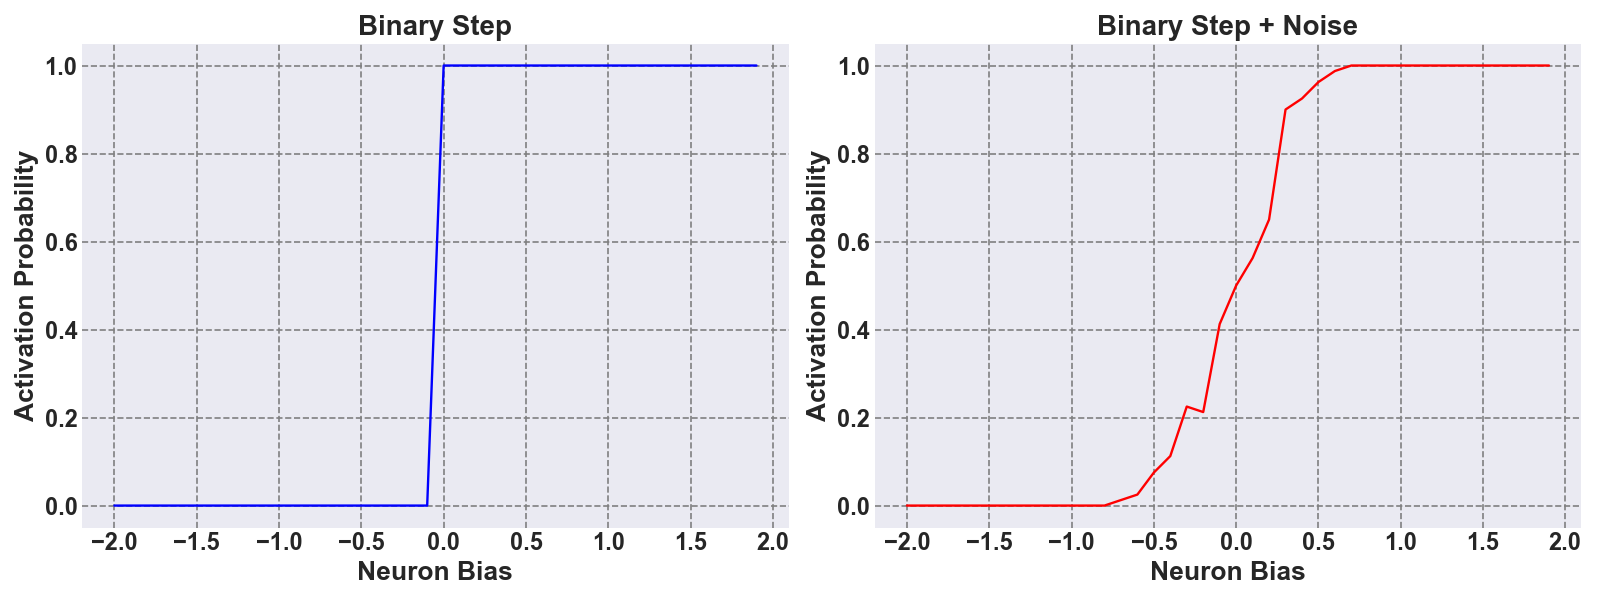
\includegraphics[width=1\linewidth]{graphics/combined_noise_activation_plots.png}
    \caption{Modification of the Hopfield Network binary step activation function}
    \label{Noisy_acitivation_function_bad}
\end{figure}
In the left plot, visualized in blue, the activation probability of the neuron is shown without adding noise to the plot. 
The behavior is like one would expect it; once the bias reaches 0 the neuron is activated all the time.
In the right figure with the red line, a noise of \(sigma=0.3\) is added.
The resulting activation is probabilistic and follows a rudimentary sigmoid shape, very similar to the activation function of a \ac{BM} shown in fig.\ref{logistic_sigmoid}.
It is visible that the noise injection works, even though it doesn't perfectly copy the sigmoid function.
Hence, the standard deviation of the noise has a direct influence on the shape of the activation function, similar to the temperature in eq.2.12. 
To correctly mimic the behavior of a \ac{BM}, it is therefore important to select the noise strength such that it corresponds to the temperature of a BM, which is \(T=1\).\footcite[cf.][3]{hintonBoltzmannMachines2014}
In the following fig.\ref{Noisy_acitivation_function_good} the standard deviation of the noise injection is optimized \(scale=1.75\) and compared to the sigmoid activation function of a \ac{BM}.
The result verifies that the \ac{mem-HNN} can correctly imitate the behavior of a \ac{BM} and its activation function:
\begin{figure}[H]
    \centering
    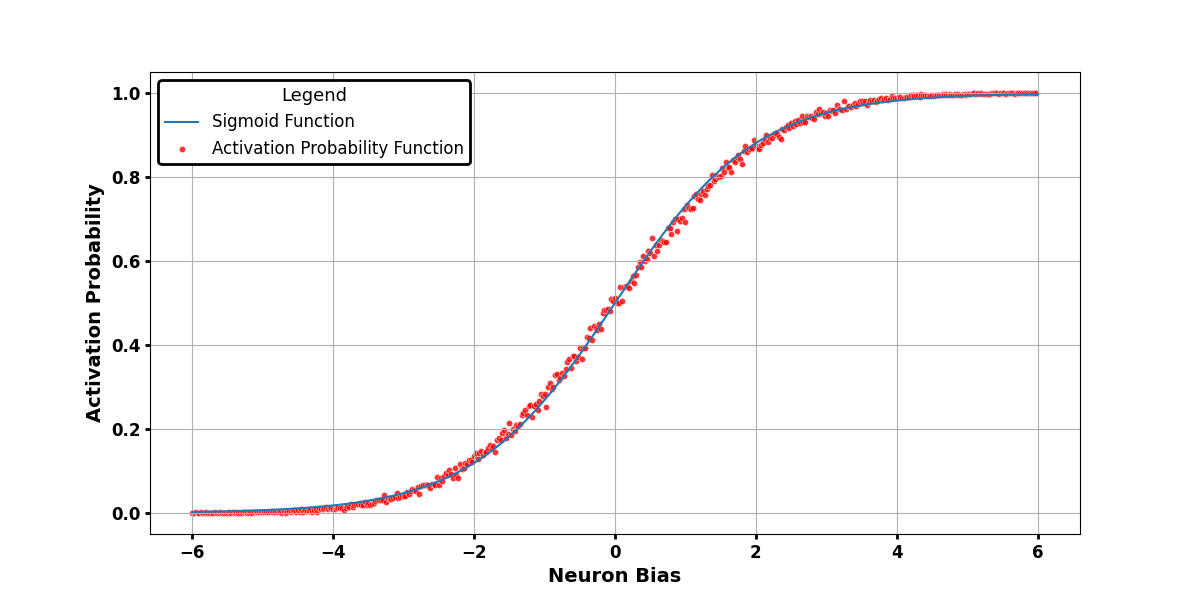
\includegraphics[width=1\linewidth]{graphics/Noisy_HNN_2.png}
    \caption{Noisy activation function of the Hopfield Network imitating the \ac{RBM}}
    \label{Noisy_acitivation_function_good}
\end{figure}
\section{Third Design and Evaluation phase}

Now, that the proof of concept has been validated, the third \textbf{Desing Phase} has the goal
integrating the \ac{mem-HNN} simulator into Scikit Learn. 
This integration enables the execution of the full Simulator Pipeline shown in fig.\ref{Overall architecture} and allows for the simulation of training a \ac{BM}.
This includes using the weights and biases of the \ac{BM} as an input and performing the sampling with the input.
Finally, the sampled output of the visible and hidden neuron configurations need to be returned, so that the digital computer can update the weights.
With these subgoals, the total goal is to enable a complete training of the \ac{BM} with the sampling method ``Hopfield Network''. 
The first technical step is to extend the \texttt{\_rbm.py} to fit the new sampling method: 
\begin{lstlisting}
        if sampling_method == SamplingMethod.GIBBS:
                v_neg = self._sample_visibles(self.h_samples_, rng)
                h_neg = self._mean_hiddens(v_neg)

        elif sampling_method == SamplingMethod.METROPOLIS_HASTING:
            h_neg,v_neg=mcmc_sample(10000,len(self.components_))

        elif sampling_method == SamplingMethod.HOPFIELD_NETWORK:  
            # Hopfield Network Sampling
            v_neg, h_neg = interface_hopfield_sampling(self.components_, self.intercept_visible_, self.intercept_hidden_, iterations_per_theta, N2_HALF=False)    
\end{lstlisting}
Here, the components represent the weights of the neurons in the network, while intercept\_visible and intercept\_hidden represent the bias of the neurons. 
Within the Hopfield network interface version 2, the parameters are taken and an object of the class is initiated. 
Furthermore, the boolean N2\_HALF can be assigned to determine which updating approach is desired. 
\begin{lstlisting}
    def interface_hopfield_sampling(components_, intercept_visible_, intercept_hidden_):
   
        H_net = Hopfield_Net(components_, intercept_visible_, intercept_hidden_)
        H_net.update_network_state()
        
        return H_net.v_neg , H_net.h_neg
\end{lstlisting}
Inside the class, the initialization of all the parameters and weights is performed. 
The update formula needs to calculate the weighted sum, which necessarily requires knowing all the weights between the neuron itself, to all the other neurons. 
The decision is to create a weight matrix shown in attachment \ref{attachement:weight_matrix}. 
The function begins by defining the total number of hidden and visible neurons based on the class properties parameters used as input.
These quantities dictate the dimensions of the weight matrix, which, in this instance, results in a matrix of size (100, 64).
This square matrix represents the fully interconnected network, where each neuron can potentially connect to every other neuron, including itself.
Again the \ac{RBM} is used as a simple test case and therefore as mentioned in 2.2.3, the diagonal elements (self-connections) are set to zero.

It is important to maintain the model's symmetry in the weight matrix, which is crucial for the energy-based nature of \ac{RBM}s and the dynamics of Hopfield networks.
Hence, for this reason a matrix is initialized as a symmetric matrix using NumPy's np.zeros function.
This ensures all initial weights are set to zero before explicitly being defined through the component's weights.
Scikit Learn randomly initializes the weights by default close to zero, while the biases are set to zero. 
These small weights allow to support of an effective gradient distribution which protects against rapid saturation or inefficient learning,
while the bias set to zero allows the network to begin in a neutral position and learn on its own. 

The subsequent nested loops iterate over the indices for hidden and visible neurons to fill the weight matrix.
For each pair of hidden and visible neurons, the corresponding weights are extracted from the components matrix.
This matrix essentially serves as the template for the interactions between hidden and visible layers.
Indexing within the weight matrix is handled carefully, to respect the structure of the \ac{BM}. 
Therefore, the decision is to set weights between a hidden neuron i and a visible neuron j at positions \texttt{[i, j+num\_hidden]} and \texttt{[j+num\_hidden, i]} to ensure symmetry.

With some more adjustments necessary to the code like transposing the returned neuron configurations, the first training with the sampling method of the Hopfield Network is possible. 
As in the Design Phase 1 the same test case of \ac{RBM} predicting on a handwritten digits classification dataset is chosen to make results comparable with the earlier established baselines.
The Hyperparmeters first are set to a scale of 1.75, thermalization of 100 as used for the single neuron in fig.\ref{Noisy_acitivation_function_good} but with more sampling steps (5000) than before. 
The results of the training are visualized in fig.\ref{HNN_training}.
\begin{figure}[H]
    \centering
    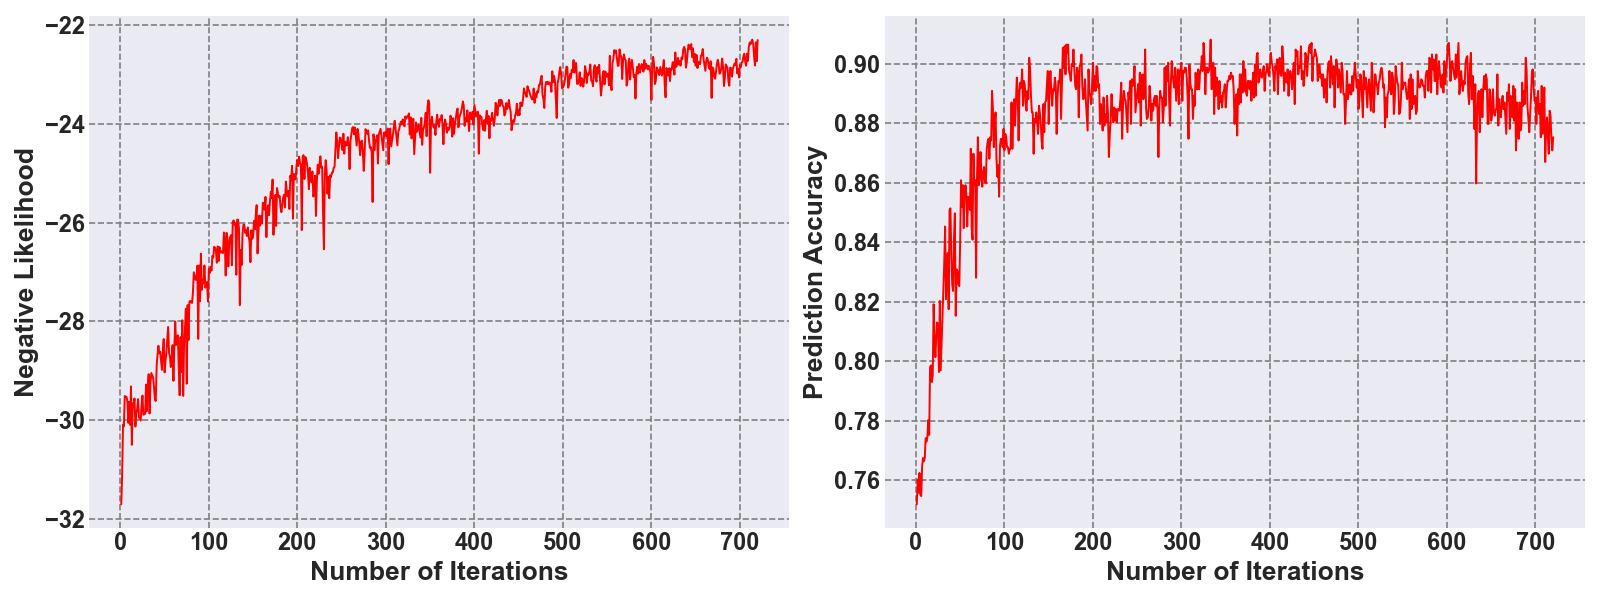
\includegraphics[width=1\linewidth]{graphics/HNN_combined_plot.png}
    \caption{Hopfield Network sampling baselines}
    \label{HNN_training}
\end{figure}
It can be seen that the negative likelihood is far more stable than Gibbs sampling and rather has similarities with Metropolis-Hastings sampling.
Here, the best value is a likelihood of -22.3, which is slightly worse than Metropolis-Hastings and Gibbs sampling. 
The right plot, which displays the prediction accuracy, shows the steepest ascent among the three graphs.
This suggests that good results can be achieved with fewer iterations compared to the other two methods.
The best prediction value is 90.81\% but no hyperparameter tuning has been done yet. 

As a result, the following hyperparameters are tuned to possibly receive better outcomes. 
Specifically, the standard deviation used for noise injection requires tuning.
In addition to that the amount of sampling iterations within a single training iteration is tuned.
Additional hyperparameters that can be tuned are the learning rate, the total amount of sampling/training iterations and the thermalization.
These are not optimized as part of this study because otherwise there is no appropriate benchmark against the other two 
sampling methods. 
First, the single neuron update Hopfield Network's hyperparameter is tuned. 
Since the training takes around 40 minutes to complete tuning too many hypaerparameters takes too much time for the period of this thesis. 
The first hyperparameter researched is the influence of the standard deviation (scale) on the maximum prediction accuracy. 
Given that the Hopfield Network operates as a statistical sampling method, the standard deviation, average and maximum are analyzed for the last 50 training iterations, as the training has stagnated at this point.
To optimize the standard deviation, it is swept from sigma=1 to sigma=2 with a stepsize of 0.05, totaling to 21 single trainings.
Lastly, only the prediction accuracy is analyzed because the negative likelihood, which represents the learning rate, is significantly steeper than the other sampling methods, and the model's final performance is of greater interest.
The result is shown in figure\ref{Hyperparamers_Scale_ohne}:
\begin{figure}[H]
    \centering
    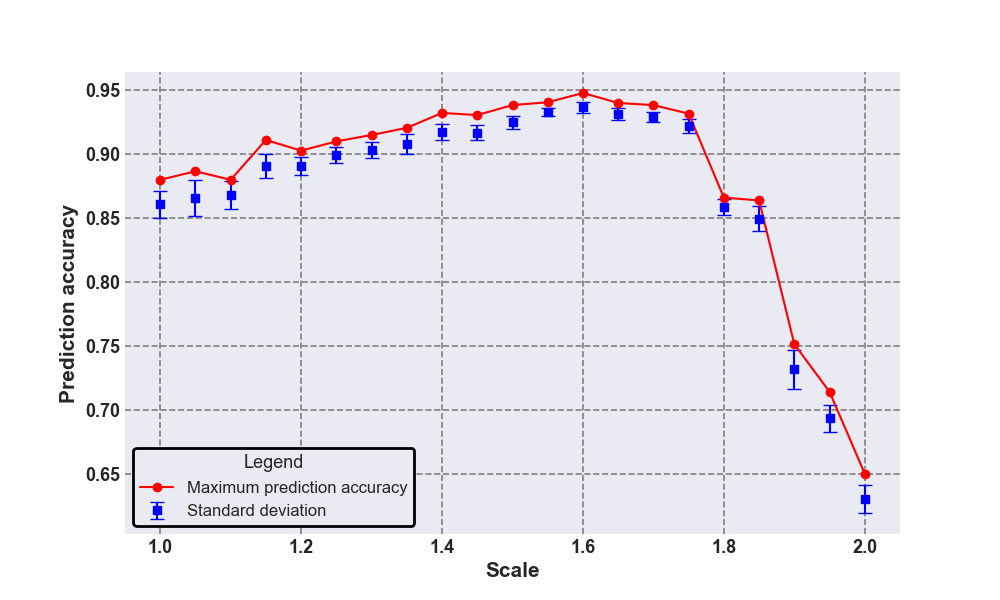
\includegraphics[width=0.9\linewidth]{graphics/NEW_Scale_Ohne_N2_Half_Pred_Acc.png}
    \caption{Hopfield Network Hyperparametertuning scale}
    \label{Hyperparamers_Scale_ohne}
\end{figure}
The result shows that beginning with a scale of 1.0 the prediction accuracy slowly rises until a scale of 1.6
Here, the maximum value is 94.77\% and with that surpasses the performance of both metropolis hastings and Gibbs sampling. 
After a scale of 1.75 the prediction accuracy rapidly declines.
This shows that with adjustments to the standard deviation, a good prediction accuracy is achievable. 
The average standard deviation follows the maximum prediction accuracy pretty closely and has no outliers.
Close to the scale of 1.0 the deviation is slightly higher compared to the rest of the plot, indicating that the scale does not model the sigmoid function correctly. 

In the next step, the best fit with a scale of 1.6 is fixed for the optimization of the number of sampling steps, as the two parameters are independent of each other. 
Hence, the decision is to begin with 1000 sampling iterations continuing with an increase of 1000 iterations until 15000 iterations are reached. 
With that, the training shows that the interesting range is around 1000 to 4000 iterations and that the step size of 1000 is too big for that. 
Therefore, additional trainings at sampling iterations 1500 and 2500 are completed, totaling to 17 trainings performed.
The values are extracted as before, by considering the last 50 iterations and then calculating both the maximum value and the standard deviation from this subset.
The visualized results can be found in the following figure\ref{Hyperparamers_Iteraions_ohne}:
\begin{figure}[H]
    \centering
    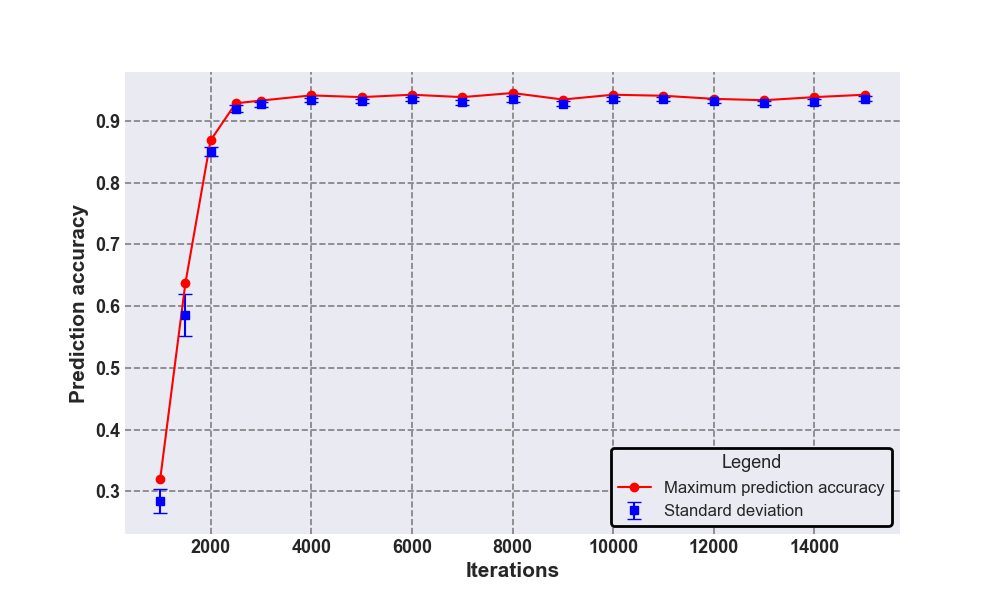
\includegraphics[width=0.8\linewidth]{graphics/Iterations_Ohne_N2_Half_Pred_Acc.png}
    \caption{Hopfield Network Hyperparametertuning sampling iterations}
    \label{Hyperparamers_Iteraions_ohne}
\end{figure}
The line of maximum prediction accuracy starts at the first iteration with a value close to 0.3 and rises rapidly to reach a value just above 0.92 after around 2500 iterations.
From the point of 4000 iterations onwards, the accuracy remains largely constant with slight fluctuations.
The best value is at 15000 iterations with a prediction accuracy of 94.5\%, while at 4000 iterations the accuracy is at 93.35\%.
The error bars indicating the standard deviation are large at the beginning of the graph.
With the number of iterations increasing, the error bars become smaller resulting in a more stable accuracy.
From this, it can be concluded that increasing the number of iterations beyond 4000 has no additional benefit to the prediction accuracy. 
In a second step the scale of N/2 Half update mechanism is analyzed and visualized in figure\ref{Hyperparamers_Scale_mit} :
\begin{figure}[H]
    \centering
    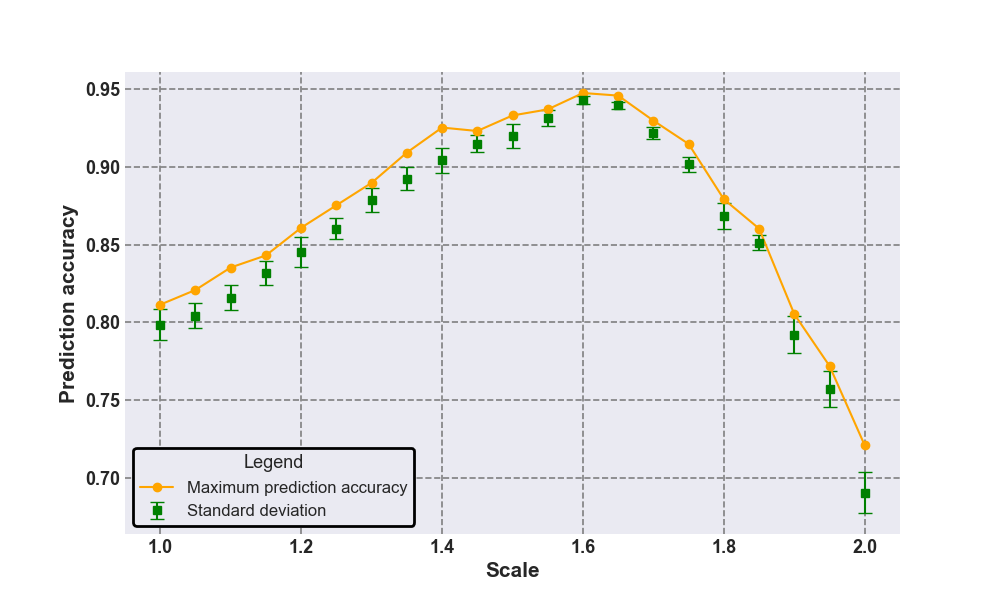
\includegraphics[width=0.8\linewidth]{graphics/NEW_Scale_MIT_N2_Half_Pred_Acc.png}
    \caption{Hopfield Network Hyperparametertuning scale for N/2}
    \label{Hyperparamers_Scale_mit}
\end{figure}
In this method, 21 complete training sessions are also carried out for this purpose
At a first glance, the prediction accuracy beginning from left to right is constantly rising until it reaches the scale of 1.6.
Here, the maximum prediction accuracy tops out at 94.76\%.
What is interesting, is that in \ref{Hyperparamers_Scale_ohne} the exact same scale has also the best performance. 
With increasing the scale after the top of 1.6, the accuracy declines rapidly. 
Noteworthy, is that in comparison with \ref{Hyperparamers_Scale_ohne} the N/2 half-updating method has nearly equal prediction accuracy
but is more sensitive. 
This means that the performance decreases more rapidly as the noise is detuned from its optimum value. 
The standard deviation represented in the error bars is high at the lower scale values but also similar for too-high values beginning at a scale of 1.8.

The second hyperparameter tuned for the N/2 Half update mechanism is the amount of sampling iterations. 
The decision is to start at iteration 201 (1st iteration after the 200 thermalization steps) and end with a sampling iteration of 250 with a step size of 1.
This totals to 50 complete training sessions. The results are illustrated in figure\ref{Hyperparamers_Iteraions_mit}:
\begin{figure}[H]
    \centering
    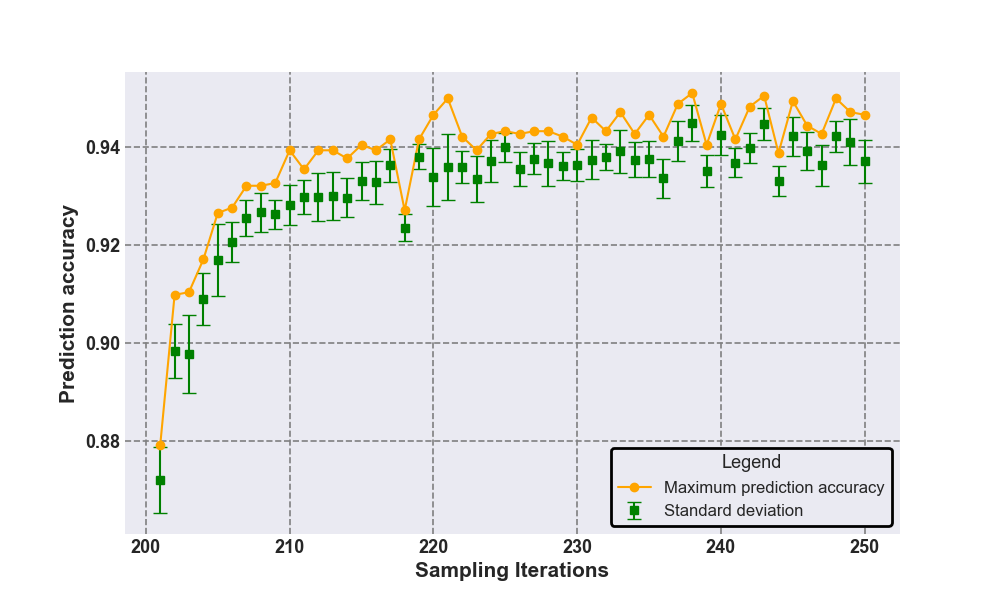
\includegraphics[width=0.9\linewidth]{graphics/Iterations_MIT_N2_Half_Pred_Acc.png}
    \caption{Hopfield Network Hyperparametertuning sampling iterations for N/2 half}
    \label{Hyperparamers_Iteraions_mit}
\end{figure}
The figure shows that with only 10 sampling iterations after the thermalization good prediction accuracies of 94\% can be achieved. 
The maximum prediction value is 95.10\% at 221 sampling iterations, which surpasses the earlier achieved results.
Nonetheless, the key result is, that far fewer sampling iterations are required within one big training iteration of the \ac{RBM}
to achieve good results. 
When comparing the number of 221 to the around 4000 sampling iterations required in \ref{Hyperparamers_Iteraions_ohne} it would be more efficient by a factor of 
\(18.09x\).
These results of the third design and evaluation pase validate that the \ac{BM}, including its weights and biases, are used as 
input to perform a complete training. 
Furthermore, the neuron configuration is returned to the digital computer to evaluate and predict the performance while updating weights and biases. 
Hence, all the functionalities of the prototype are implemented the prototype itself is complete and detailed code is available within the digital delivery. 

\section{Fourth Design and Evaluation phase}
In this final Design and Evaluation phase the goal is to enhance the \ac{mem-HNN} simulator to
predict the performance of a future \ac{mem-HNN} chip.
This equals with the goal of ultimately answering the research question ``Can Boltzmann Machines be \textbf{efficiently} implemented on physics-inspired
Hardware accelerators by analog noise injection?''.
The \textbf{Design} phase enables this by implementing the energy model and an autocorrelation metric on top of the functional Simulator.
Since the keyword is efficiently, this happens in the methodology of a simulation, which requires specifying the parameters measured for evaluation.
With the model purpose set, the model scope(time frame) of the simulation introduced in 3.4 is to be considered as short with only multiple weeks and only one person working on the simulation. 
The next step is to define the result variables. The two variables that are of interest in literature to ensure the performance of the
\ac{mem-HNN} accelerator is throughput (samples/sec) and energy consumption (energy/operation). 
These two metrics are widely used in literature and can create a good comparison.\footnote{cf.\cite{bellettiJanusFPGABasedSystem2009}, p. 54-55; cf.\cite{aaditAcceleratingAdaptiveParallel2023}, p. 1-2; cf.\cite{ortega-zamoranoFPGAHardwareAcceleration2016}, p. 16-17}
Hereby, throughput can be defined as the time needed per Hopfield cycle (sampling iteration) per second.\footcite[cf.][6-7]{bohmNoiseinjectedAnalogIsing2022} 
Meanwhile, energy consumption is defined by summing over all the single energy consumptions within one sampling iteration.
The resulting unit is called energy/operation. 

Now that the result variables are set the input parameters need to be clarified. 
For the throughput knowledge about the autocorrelation of the sampling is required.
Autocorrelation is a statistical measure that captures the degree of correlation between successive configurations generated by time series, in this case, sampling algorithm for the training of a \ac{RBM}.\footcite[cf.][1-6]{tanakaReductionAutocorrelationHMC2017}
Long correlations between configurations can reduce the effective sample size and lead to inefficiency impacting the precision of the model.
This is important for the result variable ``throughput'' because it allows to know when the sampling is statistically independent and ready to use and therefore how many sampling iterations need to be done for effective training. 
Combined with the specifications of the chip it can be calculated what the resulting throughput is.
Here, covariance is implemented and used to measure the correlation between two successive samples:
\begin{equation}
    K_{XX}(t_1, t_2) = \mathbb{E}[(X_{t_1} - \mu_{t_1})(X_{t_2} - \mu_{t_2})] = \mathbb{E}[X_{t_1} X_{t_2}] - \mu_{t_1}\mu_{t_2},
\end{equation}
with \(t_1,t_2\) being two distinct points in time and \(X_{t1},X_{t2}\) are random variables representing the values of the stochastic process at the distinct time points. 
\(\mu_1,\mu_2\) are the mean (expected) values of the random variables \(X_{t1},X_{t2}\). 
The \(\mathbb{E}\) is an expectation operator and is used to calculate the expected value of the expression within the brackets.
Also, the cycle speed of the \ac{mem-HNN} accelerator is needed. 
The cycle time is based on the simulation shown in ref\footcite[cf.][4]{hizzaniMemristorbasedHardwareAlgorithms2023}, where a single Hopfield update cycle is performed in a single clock cycle with a frequency of 700 MHz, resulting in a cycle time of 1.44ns.
With the simulation model specified, the autocorrelation is implemented into the prototype. 
The changes made for the implementation of the autocorrelation are available in the interface version 5 and part of the digital delivery. 

Next, the only input variable to measure the second metric \textbf{energy consumption} is the energy model, which is introduced in 4.2.1 and is developed by HPE in combination with the Forschungszentrum Jülich.
The implementation of it allows us to measure each of the individual energy consumptions that are configured to the specifications of the \ac{mem-HNN} hardware accelerator.\footcite[cf.][1-5]{hizzaniMemristorbasedHardwareAlgorithms2023}
The energy function is provided in the form of a Python library, that returns the average energy consumed for a single clock cycle.
Specifically, it includes functions to calculate the energy usage of the probabilistic random number generator, the register, the crossbar and the digital-analog converter that generates the noise signal.
These functions are based on circuit simulations that were performed on a 28nm technology node that can be fabricated with commercial foundry services.
As input, the energy model requires the number of neurons, the average activation rate and the output pattern rate during a single clock cycle.
Hence, the mentioned energy model needs to be implemented into the Hopfield Network interface.
The first implementation is to \textbf{intialize the energy model} with the size of 164 neurons as this impacts the size of the crossbar array and influences the overall energy consumption.
An increase in the number of neurons causes a higher energy consumption due to the enlarged crossbar structure.

Afterward, the two parameters ``a\_pattern'' and ``a\_WL'' need to be calculated.
Hereby, a\_pattern refers to the currents that flow through the respective bitlines (output pattern rate).
The current for each bitline is determined by the average of the weighted sum and is accumulated with each iteration.
Subsequently, it is divided by the number of sampling iterations to obtain an average for the respective training iteration.
For a correct calculation and imitation of the \ac{mem-HNN}, there is one more restriction to solve. 
The digital computer generates negative and positive weights and biases, which is not possible in the hardware.
Therefore, the weight matrix is adjusted to handle positive and negative weights separately. 
Lastly, the memristors can be tuned to a limited amount of discrete conductance levels.
For the \ac{mem-HNN} design, the memristors can be set to around 32 different levels, which correspond to a 5-bit resolution. 
Due to this, the coupling matrix of the \ac{BM} is discretized to this resolution, where the lowest conductance level corresponds to the highest weight value.
In earlier design phases, the values are calculated with perfect resolution but for the energy model, this is not possible anymore. 
A\_Wl is the average configuration change (average activation rate).
This parameter tracks the average changes in configuration within the wordline.
Each time the state changes from 0 (no current) to 1 (current flows), energy is consumed by the switching process.
To calculate the average energy consumed by such switching processes, the average number of rising bits is measured between subsequent iterations.
Subsequently, an average change rate is calculated by dividing by the number of iterations.
This approach quantifies the energy cost associated with state transitions within the network configuration.
All the implementations for the energy model within the interface can be found in version 5 of the Hopfield interface as part of the digital delivery.

Of course, for both the energy model and the autocorrelation the methods one input is the finished prototype, that mirrors the functionalities of the \ac{ASIC} on a high level.
The first \textbf{Evaluation} focuses on the throughput, which is decided to average the values of the output configurations from row to row to an average of 60.
This allows to extract of a smoother autocorrelation plot.
In the attachment\ref{attachement:autocorrelation} the full implementation of the autocorrelation function is available.
To compare the performance of the sampling methods in terms of the autocorrelation a threshold is required. 
Here, \(1/\mathrm{e}\) is chosen since it is inspired by many fields, like physics(diffusion length), chemistry(half-life as a threshold) etc..\footnote{cf.\cite{archieStatisticalAnalysisHeterozygosity1985}, p. 624-630; cf.\cite{bohmNoiseinjectedAnalogIsing2022}, p. 7-13}
Following results can be \textbf{evaluated} and are shown in following figure\ref{Autocorr comparison}:
\begin{figure}[H]
    \centering
    \includegraphics[width=0.95\linewidth]{graphics/Visualisierungen_Autocorr_individual_7.png}
    \caption{Autocorrelation for the three sampling methods}
    \label{Autocorr comparison}
\end{figure}
The first row shows the conventional \textbf{Metropolis Hastings} sampling method. On the right plot the autocorrelation
and the according sampling steps are visualized for the first training iteration.
It can be seen, that the value falls below the threshold at around \textbf{100 sampling steps}.
Falling below the threshold of \(1/\mathrm{e}\) symbolizes that statistically independent samples are generated.
The left plot therefore measures the correlation time time within each training iteration, where these samples are first generated. 
It can be seen that the the scale on the x-axis in the left plot is higher compared to the other two sampling approaches, 
meaning that metropolis hastings is \textbf{more sensitive}. 
The second row is the \textbf{single update Hopfield Network} sampling approach. 
In the right plot, it shows that the autocorrelation threshold reached around \textbf{200 sampling steps}.
Even if the value is \textbf{2x worse} than with metropolis Hastings the correlation time for the whole training is \textbf{more stable}.
So even if the initial autocorrelation takes longer over a whole training period the end result has an \textbf{better average} than Metropolis-Hastings.

The last approach is the \textbf{N/2 half Hopfield Network}. 
This method only needs about \textbf{3 iterations} to surpass the threshold in the right plot.
Furthermore, the method correlation time in the left plot shows that it is by far more \textbf{stable} than the other 2 approaches.
When setting this into perspective even with a conservative average of 5 iterations as correlation time, N2/Half updating therefore
performs \textbf{40x better}, than the single neuron Hopfield Network and \textbf{20x better} than Metropolis Hastings.
When comparing the correlation at the end of the training iterations, the performance even increases: \textbf{34x better} than the single neuron Hopfield Network (correlation time value of 170) and \textbf{46,6x better} than Metropolis Hastings (correlatin time value of 233).
Surprisingly for this updating method large statistical dependency could be seen in two out of the 720 training iterations.
This means that for these two iterations the autocorrelation \textbf{doesn not fall under the threshold} of \(1/\mathrm{e}\).
The training was attempted three times, and in each instance, the phenomenon occurred between iterations 300 and 500.
Still, this has no impact on the performance of the training and therefore can be seen as an outlier.
It is open for further research to identify why this does not happen with the other two approaches and what is the cause.
As the corresponding correlation time for the outliers is infinite, the scale has been reduced here for better visualization of other data points.

Based on this implementation, the desired ``throughput'' of the simulator, which reflects the rate at which statistically independent samples are generated, is calculated.
This is done by combining the autocorrelation time of both Hopfield Network approaches (with N/2 Half and without) and multiplying them with the cycle speed of the \ac{mem-HNN}.
Then, the inverse of the result is calculated resulting in the desired throughput metrics `` samples/second''.
The simulation was conducted using a network of 111 neurons.\footcite[cf.][4]{hizzaniMemristorbasedHardwareAlgorithms2023}
However, it is assumed that for the 164 neurons utilized in this thesis, the clock frequency is reduced.
This is because a larger crossbar has a longer delay.
As a first assumption, the cycle time scales linearly with the number of neurons and therefore reaches a clock frequency around \textbf{2ns} for 164 neurons.
Because the network in this thesis has 164 neurons, the time used for the calculation is estimated to be about 2ns, which can be seen as a conservative estimate.
The subsequent visualization\ref{Throughput comparison} shows the throughput for the Hopfield Network:
\begin{figure}[H]
    \centering
    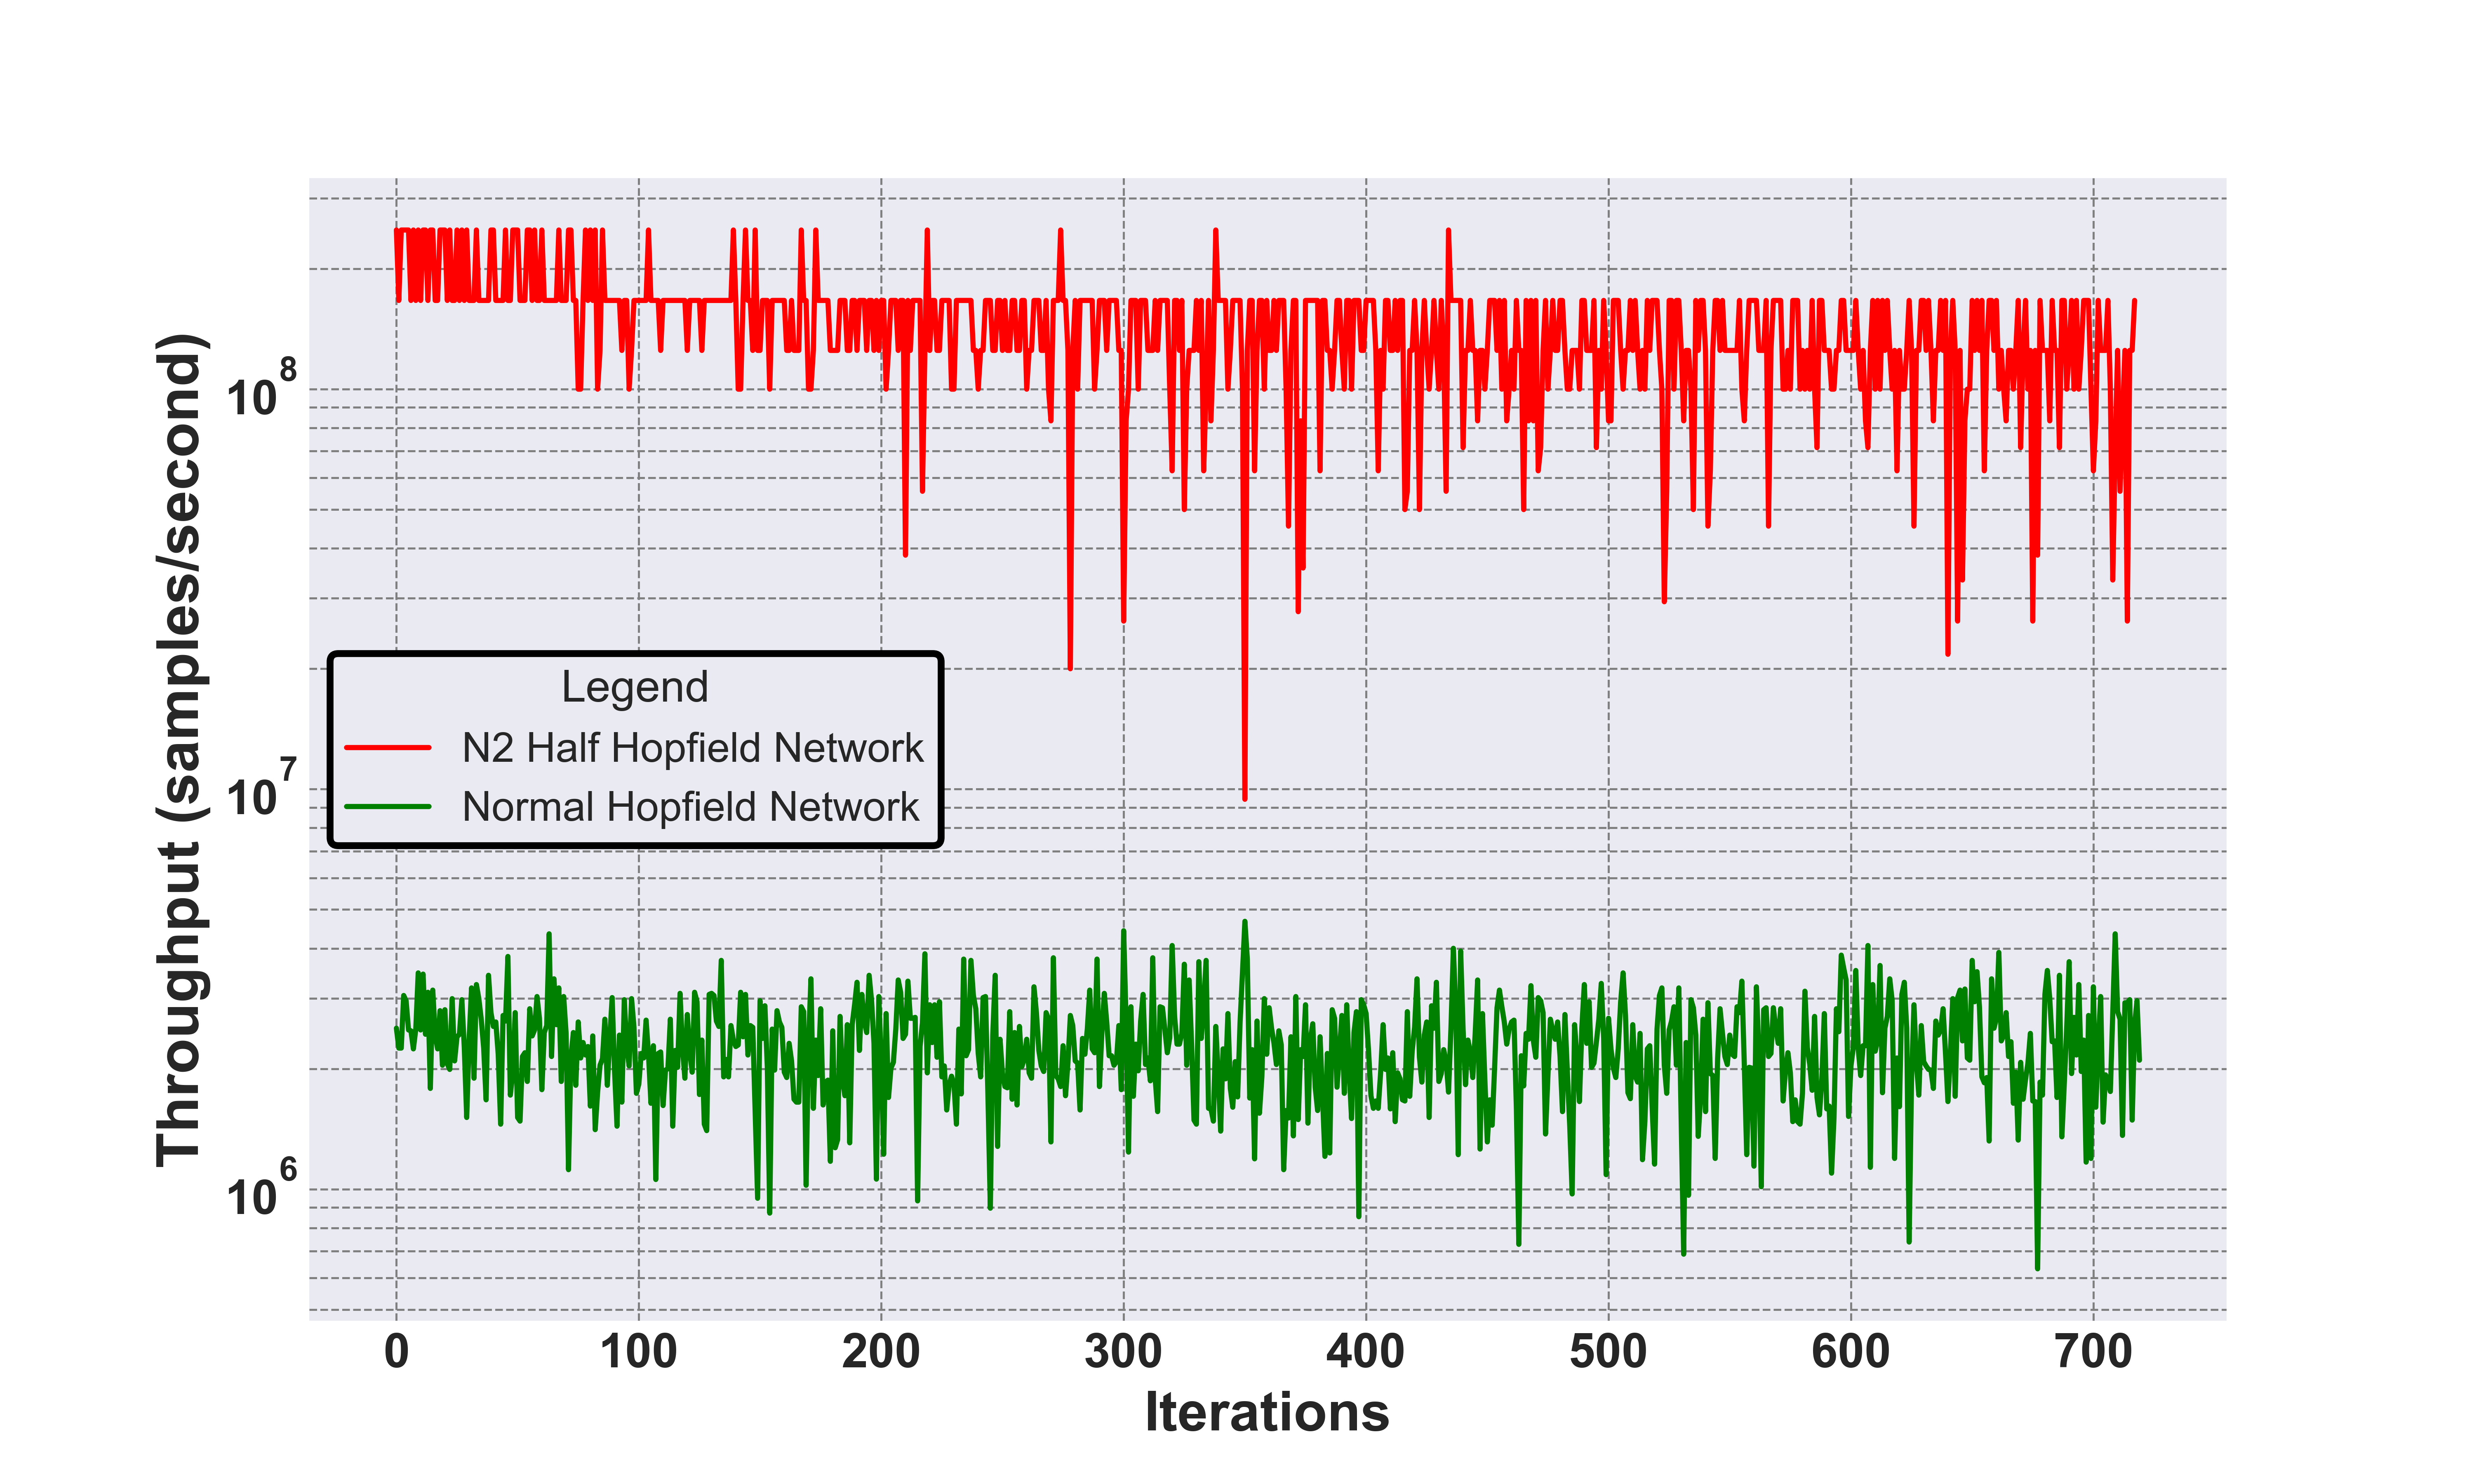
\includegraphics[width=0.7\linewidth]{graphics/Visualisierungen_throughput_log_2.png}
    \caption{throughput for Hopfield network}
    \label{Throughput comparison}
\end{figure}
The following results of the two networks show that the Hopfield Network (green line) maintains stable throughput at over \(\mathbf{10^6}\) samples per second, indicating predictable performance.
In contrast, the N2 Half Hopfield Network (red line) shows greater variability, typically ranging from \(\mathbf{10^8}\) \textbf{to} \(\mathbf{10^9}\) samples, but fluctuates more than the single update approach.
Calculating the average throughput, the N/2 Half Hopfield Network achieves \textbf{144 megasamples/second}, significantly outperforming the Hopfield Network's \textbf{2,3 megasamples/second}.
This means that the computation speed of the N/2 Half method \textbf{is faster} by a factor of \textbf{62.72x}.
In general, this shows that the N/2 Half update can considerably increase the computing speed in the sampling of neuron activation probabilities and
implies a low energy consumption.
The next \textbf{evaluation} focuses on the energy consumption, which is shown in the following fig.\ref{Energy output_2}:
\begin{figure}[H]
    \centering
    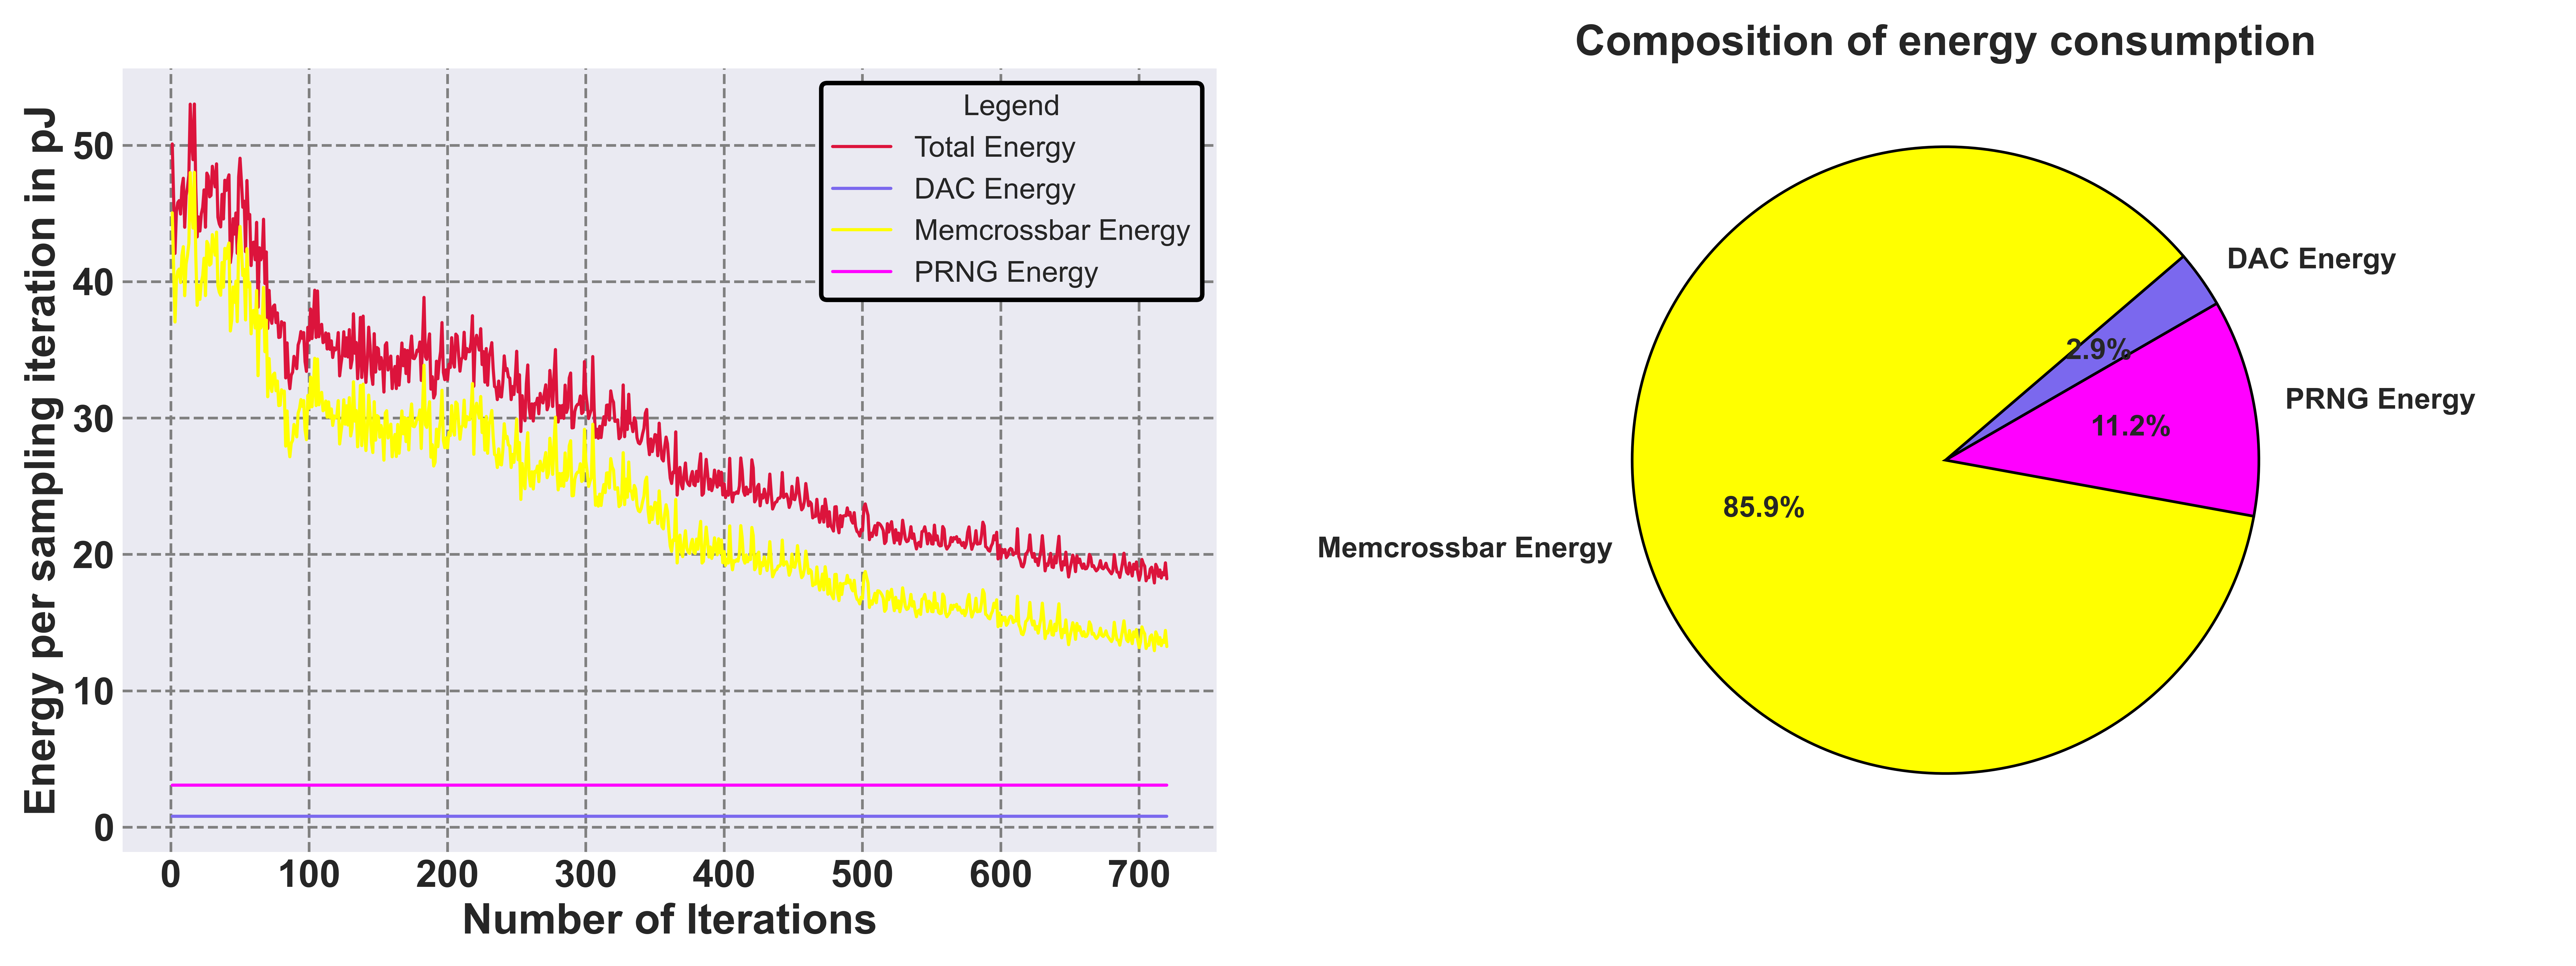
\includegraphics[width=0.9\linewidth]{graphics/energy_and_averages_plot_4.png}
    \caption{Energy consumption of the \ac{mem-HNN}}
    \label{Energy output_2}
\end{figure}
The left plot shows the energy consumed per sampling iteration in pico Joules.
At the beginning of the training, the average clock cycle has a total energy consumption of around 45 pico Joules.
Further in the training at around 100 training iterations, the consumption drops to around 35 pico Joules. 
At the end of the training, the value falls just below the 20 pico Joules mark. 
This decrease may be attributed to the network's weights reducing on average, impacting a\_pattern.
The Memcrossbar is the primary variable energy consumer, while the digital-to-analog converter and pseudo-random number generator remain constant. 
A composition of the energy consumption is shown in the right plot.
It is important to note that the plot does not include all hardware components,
specifically the communication with the memory, the controller of the \ac{mem-HNN}, and the updating of weights in the digital computer.
While the sampling is the computationally most demanding task in the training, it can still be expected that these components consume additional energy.

In the next step, the power consumption of the training is targeted as this delivers a good comparison to other
hardware components like \ac{CPU}s, \ac{GPU}, \ac{ASIC}s or \ac{FPGA}s.
Therefore, the energy per sampling iteration is divided by the time of one clock cycle (2ns) since \(P = \frac{\Delta E}{\Delta t}\).
Furthermore, the right plot in fig.\ref{Power consumption} is based on the power and cumulates the power multiplied with the sampling iteration to visualize how much energy the training of neural network consumes for this workload.
\begin{figure}[H]
    \centering
    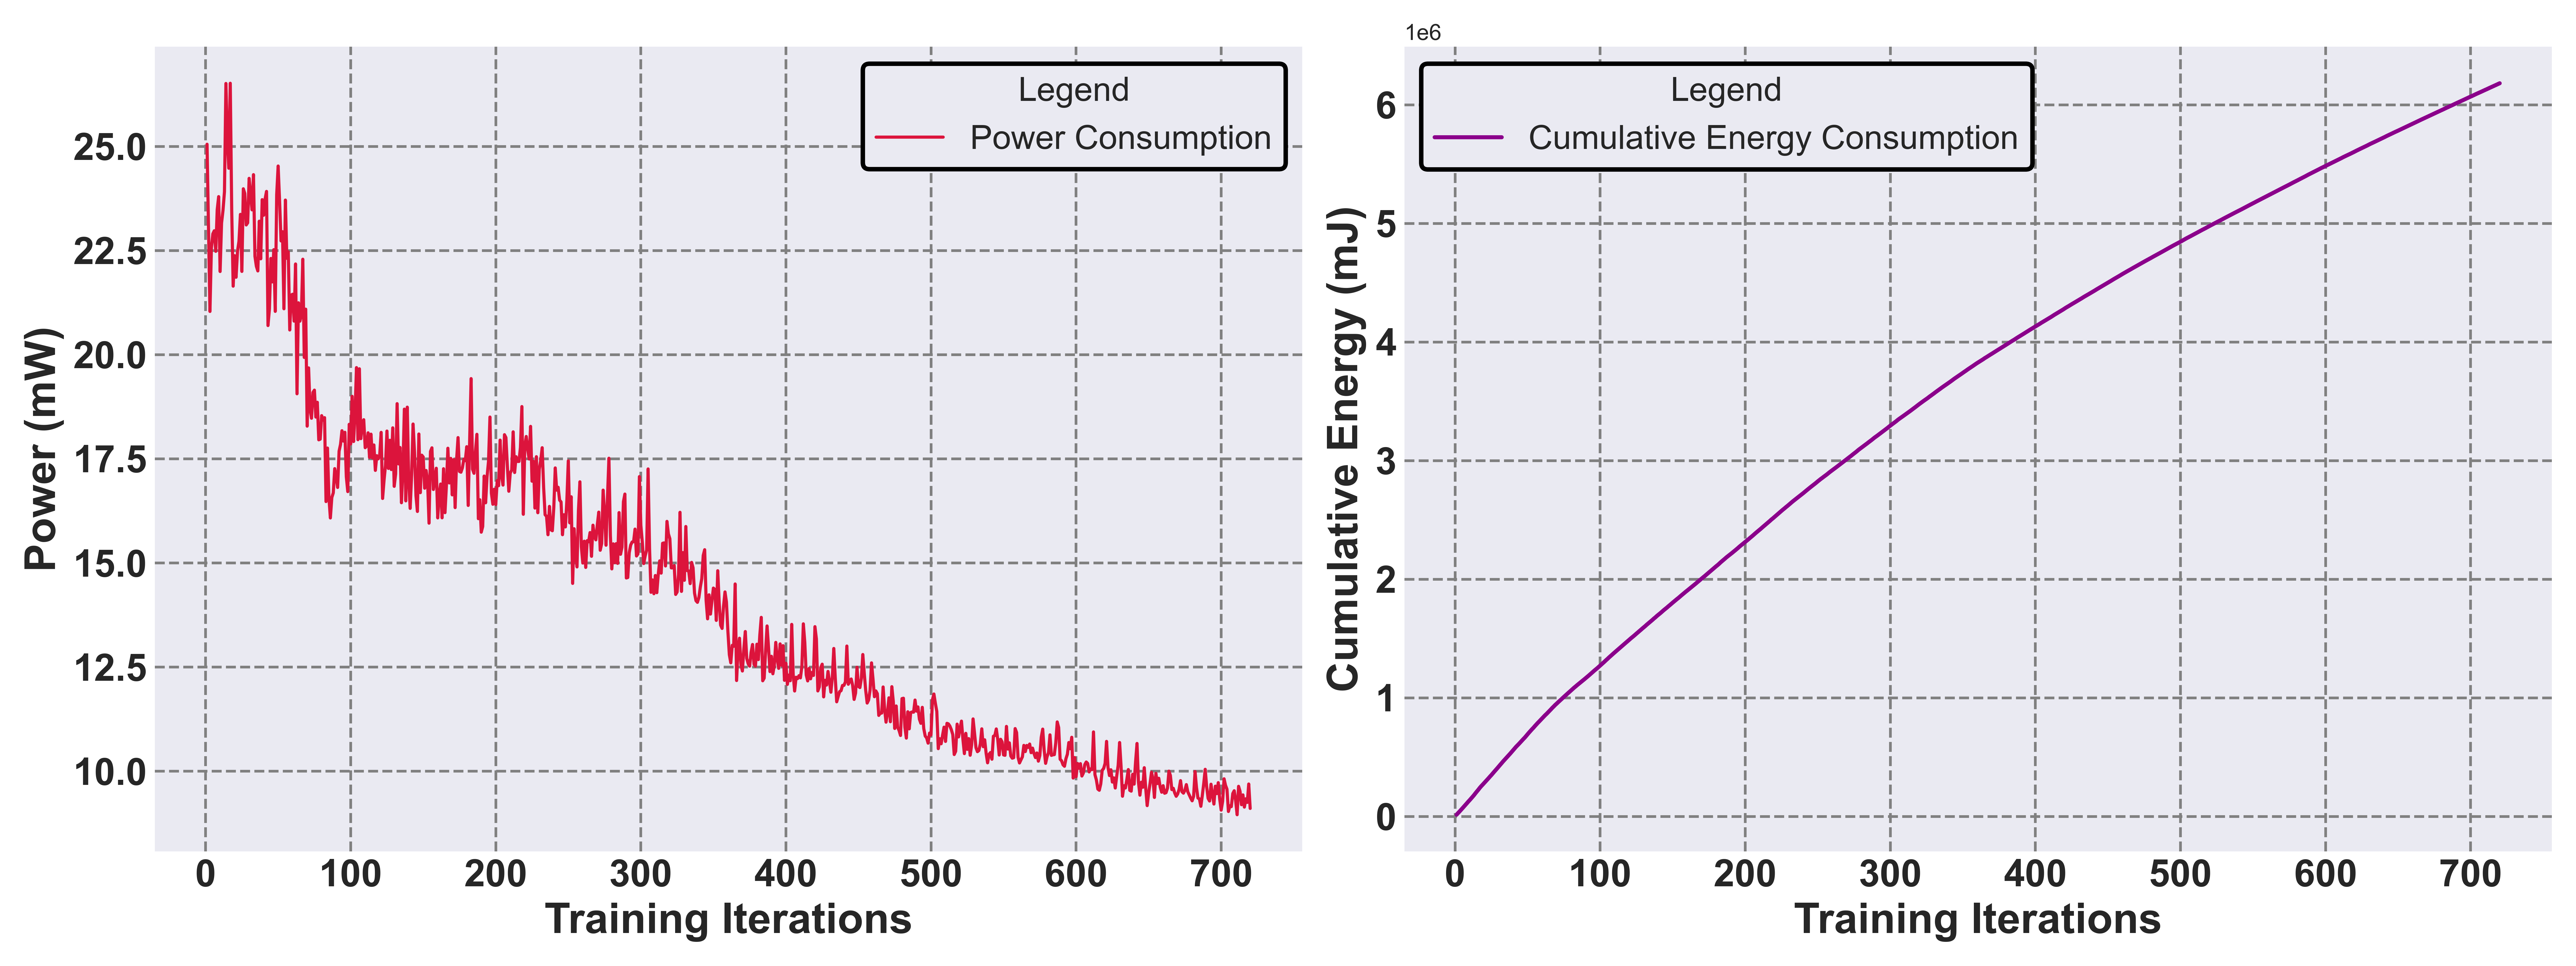
\includegraphics[width=0.9\linewidth]{graphics/energy_consumption_cumulative_plot.png}
    \caption{Power consumption of the \ac{mem-HNN}}
    \label{Power consumption}
\end{figure}
Figure \ref{Power consumption} reveals that training requires a maximum of 22.5 mW, substantially less than a basic CPU (20-40W); but for an accurate comparison, OS overhead should be excluded and measurements conducted using tools like Powertop.\footcite[cf.][1]{PowertopArchWiki} 
Again with training iterations continuing to grow the power consumption decreases. 
At the end of the training around 620 iterations, a power consumption of around 10mW is reached. 
The power consumption is mostly stable with some minor fluctuations in the beginning.
When looking at the right plot, shows the cumulative energy required for the training in mJ.
Here, it is visible that a complete training with 720 iterations requires around 6.2 mJ. 
With that, the evaluation phase can successfully verify the model's purpose of the simulation, which is to measure the performance of the \ac{mem-HNN}.
The gathered data can be used in the next chapter to compare the efficiency with conventional hardware but the
the first part of the research question is already answered within the iterative design and evaluation phases of the \ac{DSR} framework.
